\documentclass[a4paper, 11pt]{report}%choice of the class of the document
\usepackage[french]{babel}%choice of language
\usepackage{amssymb,bm,graphicx,graphics,subfigure,geometry}%different packages
\usepackage[breaklinks]{hyperref} % for appendix and label
\usepackage[final]{pdfpages}%insertion of pdf
\usepackage{url}%format adress url
\usepackage{fancyhdr}% header and footer can be modified
\usepackage[official]{eurosym}% symbol of money euro. for dollar tape : \$
\usepackage{textcomp}%special letter
\usepackage{parskip}% for paragraph and skip
\usepackage[version=4]{mhchem}% for chemistry
\parskip=0.1in% for chemistry
\usepackage[italic]{hepnames} % for proton etc 
\usepackage{mathtools} % for math symbol
\usepackage{amssymb,amsmath}% for insert math eq in latex
\usepackage{qtree} % to create trees
\usepackage{color} % color the text

%********************************************************
%for side by side figure
\usepackage{subfigure}

%*********************************************************
%for changing size section, subsection etc
%\usepackage{titlesec}

%\titleformat*{\section}{\LARGE\bfseries}
%\titleformat*{\subsection}{\Large\bfseries}
%\titleformat*{\subsubsection}{\itshape\bfseries}
%\titleformat*{\paragraph}{\large\bfseries}
%\titleformat*{\subparagraph}{\large\bfseries}

%*********************************************************
%for drawing in latex
\usepackage{tikz}
\usetikzlibrary{arrows,shapes,trees,backgrounds,positioning,shadows}

\tikzset{
  %basic/.style  = {draw, drop shadow},%font=\sffamily,
  root/.style   = {drop shadow, rounded corners=2pt, thin, align=center,
                   fill=green!75},
  level 1/.style = {drop shadow, rounded corners=6pt, thin,align=center, fill=green!65},
  level 2/.style = {drop shadow, rounded corners=6pt, thin,align=center, fill=green!60},
  level 3/.style = {drop shadow, rounded corners=6pt, thin,align=center, fill=green!55},
  level 4/.style = {drop shadow, rounded corners=6pt, thin,align=center, fill=green!50},
}


%***********************************************************
%for overwite on picture
\usepackage[percent]{overpic}

%**********************************************************
%for degree symbol
\usepackage{gensymb}

%**********************************************************
%for color text
\usepackage{color}%for color on text

%**********************************************************
%for fancy table
%\usepackage[usenames,dvipsnames]{xcolor}
\usepackage{tcolorbox}
\usepackage{tabularx}
\usepackage{array}
\usepackage{colortbl}
\tcbuselibrary{skins}

\newcolumntype{Y}{>{\raggedleft\arraybackslash}X}

\tcbset{tab1/.style={ fonttitle=\bfseries\large, fontupper=\normalsize\sffamily, colback=yellow!10!white, colframe=red!75!black,
  colbacktitle=blue!40!white, coltitle=black, center title, freelance,
  frame code={ \foreach \n in {north east,north west,south east,south west}
  {\path [fill=red!75!black] (interior.\n) circle (3mm); };},}
}

\tcbset{tab2/.style={enhanced, fonttitle=\bfseries, fontupper=\normalsize\sffamily,
  colback=yellow!10!white, colframe=red!50!black, colbacktitle=blue!40!white,
  coltitle=black,center title,totalheight = 0.2\textwidth}}
  
  
\newgeometry{top=2.5cm,right=3cm,left=2cm,bottom=2.5cm}

%%%%%%%%%%%%%%%%%%%%%%%%%%%%%%%%%%%%%%%%%%%%%%%%%%%%%%%%%%%%
%     few commandes to control geometry of paper :         %
% https://www.sharelatex.com/learn/Page_size_and_margins   %
%%%%%%%%%%%%%%%%%%%%%%%%%%%%%%%%%%%%%%%%%%%%%%%%%%%%%%%%%%%%

%\usepackage[a4paper, top=25mm, bottom=2mm, left=25mm, right=15mm]{geometry}
%\sloppy
%\addtolength{\headheight}{-2.0cm}
%\addtolength{\textheight}{+2.0cm}
%\addtolength{\oddsidemargin}{-0.5cm}
%\addtolength{\textwidth}{+1.0cm}

\setlength{\parindent}{15pt}%set alinea of paragraph. Default 15 pt. 


\newcommand{\TPS}{T\'\'el\'\'ecom Physique Strasbourg }
\newcommand{\PLG}{P. LOPES GOMES }
\newcommand{\IR}{Internship Report}
\newcommand{\TotI}{Photo-detector development for nEXO}
\newcommand{\xfl}{Flash lampe au X\'enon }
\newcommand{\TR}{TRIUMF }
%\newcommand{\(0\Pneutrino\beta\beta\)}{0$\Pneutrino\beta\beta$} % \(0\Pneutrino\beta\beta\)
%\newcommand{\(2\Pneutrino\beta\beta\)}{\(2\Pneutrino\beta\beta\)} % \(2\Pneutrino\beta\beta\)

\newcommand*{\fullref}[1]{\hyperref[{#1}]{\autoref*{#1} \nameref*{#1}}} % One single link

%%%%%%%%%%%%%%%%%%%%%%%%%%%%%%%%%%%%%%%%%%%%%%%%%%%%%%%%%%%%
%             fancy header and footer                      %
%%%%%%%%%%%%%%%%%%%%%%%%%%%%%%%%%%%%%%%%%%%%%%%%%%%%%%%%%%%%

%\pagestyle{headings}%style classique.
%\pagestyle{fancy}%style for paper.Can be modified if necessary. 

%%%% fancy header %%%%
%\fancyhead{}%empty pre-defined header parameters
%\fancyhead[L]{\TotI}
%\fancyhead[L]{\slshape \rightmark}% seem to copy main subtitle of chapter
%\fancyhead[R]{\PLG Rapport 2015}% date
%\renewcommand{\headrulewidth}{0.4pt}%add a line of 0.4 pt under header 

%%%% fancy footer %%%%
%\fancyfoot{}%empty pre-defined footer parameters
%\fancyfoot[L]{\IR} 
%\fancyfoot[C]{\PLG}
%\fancyfoot[R]{\thepage}% number of page
%\renewcommand{\footrulewidth}{0.4pt}%add a line of 0.4 pt above footer

\renewcommand{\thefootnote}{\arabic{footnote}} % Arabic numerals
%\fontfamily{fi4}\selectfont

\renewcommand{\footnoterule}{%
  \kern -3pt
  \hrule width \textwidth height 1pt
  \kern 2pt
}

%%%%%%%%%%%%%%%%%%%%%%%%%%%%%%%%%%%%%%%%%%%%%%%%%%%%%%%%%%%%
%%%%%%%%%%%%%%%%%%%%%%%%%%%%%%%%%%%%%%%%%%%%%%%%%%%%%%%%%%%%
%%%%%%%%%%%%%%%%%%%%%%%%%%%%%%%%%%%%%%%%%%%%%%%%%%%%%%%%%%%%
%%%%%%%%%%%%%%%%%%%%%%%%%%%%%%%%%%%%%%%%%%%%%%%%%%%%%%%%%%%%

%%%%%%%%%%%%%%%%%%%%%%%%%%%%%%%%%%%%%%%%%%%%%%%%%%%%%%%%%%%%
%                     begin document                       %
%%%%%%%%%%%%%%%%%%%%%%%%%%%%%%%%%%%%%%%%%%%%%%%%%%%%%%%%%%%%

\begin{document}

%%%%%%%%%%%%%%%%%%%%%%%%%%%%%%%%%%%%%%%%%%%%%%%%%%%%%%%%%%%%
%                     cover page                           %
%%%%%%%%%%%%%%%%%%%%%%%%%%%%%%%%%%%%%%%%%%%%%%%%%%%%%%%%%%%%


\includepdf{page_couverture_TPS.pdf}

%%%%%%%%%%%%%%%%%%%%%%%%%%%%%%%%%%%%%%%%%%%%%%%%%%%%%%%%%%%%
%                chapter 1 Introduction                    %
%%%%%%%%%%%%%%%%%%%%%%%%%%%%%%%%%%%%%%%%%%%%%%%%%%%%%%%%%%%%

\newpage
\thispagestyle{empty}

\paragraph{\textit{\underline{Introduction}}}
  \leavevmode
  \\
  
  J'ai effectu\'e mon stage de fin d'\'etude \`a \TR. Situ\'e \`a Vancouver au Canada, \TR est un laboratoire de recherche sur la physique 
  nucl\'eaire et la physique des particules.Comme tous les laboratoires de recherche, \TR accueille d'autres exp\'eriences dont 
  l'exp\'erience nEXO.\\
  
  Le but de nEXO est de mettre en \'evidence que la particule \'elmentaire -le neutriono- est une particule de Majorana. Pour cela nEXO 
  utilise une d\'esint\'egration b\^eta: la d\'esint\'egration double b\^eta sans \'emission de neutrino. Plusieurs \'el\'ements chimiques, dont le 
  X\'enon, peuvent donner lieu \`a cette d\'esint\'egration: 
  
  \begin{equation}\label{eq:beta}
    \ce{^{136}Xe} \rightarrow \ce{^{136}Ba} + 2\Pelectron
  \end{equation}

  L'exp\'erience est donc constituer d'un cuve contenant 5 tonnes de X\'enon liquide. Les \'electrons \ref{eq:beta} \'eject\'ees avec une grande 
  \'energie cin\'etique peuvent percuter d'autres \'electrons li\'es \`a d'autres atomes de X\'enon. Ces derniers, alors exit\'es, vont se d\'esecit\'es
  en emettant de la lumi\`ere (photon). La lumi\`ere produite a une longueur d'onde de 175 nm. 
  \\
  
  Pour mesurer, avec une grande pr\'ecision, 
  cette \'energie de scintillation, nEXO \'etudie des photo-d\'etecteurs qui doivent satisfaire trois conditions:\\
  1) l'efficacit\'e quantique (PDE) doit \^etre sup\'erieur \`a 15$\%$, 2) le bruit thermique doit \^etre inf\'erieur \`a 50Hz/mm\textsuperscript{2},
  3) le nombre moyen d'impulsions corr\'el\'ees \`a une impulsion primaire doit \^etre inf\'erieur \`a 0.2 par impulsion primaire. 
  \\
  
\paragraph{\textit{\underline{Photo-d\'etecteurs au silicium (SiPM)}}}
  \leavevmode
  \\
  
  Les SiPMs sont des photo-d\'etecteurs, constitu\'es d'une matrice de pixels. Chaque pixel est une photodiode \`a avalanche fonctionnant en 
  mode Geiger. Quand un/des photon(s) traverse(nt) la surface d'un pixel, il(s) d\'eclenche(nt) \`a l'int\'erieur de celle ci une/des avalanche(s)
  de pairs de porteurs de charges (\'electrons et trous). Le signal issue de ce courant d'avalanche(s) provenant d'un pixel est 
  caract\'eris\'e par une impulsion (dite impulsion primaire).
  Le courant d'avalanches est ensuite coup\'e gr\^ace \`a une r\'esistance \footnote{Dite r\'esistance de shunt.} et le pixel est de nouveau pr\^et pour
  \^etre irradi\'e. 
  \\
  
  Trois probl\`emes principaux sont li\'es \`a l'utilisation de tels d\'etecteurs:
  
  \begin{itemize}
   \item Le bruit thermique. Des porteurs de charges sont g\'en\'er\'es thermiquement \`a l'int\'erieur d'un pixel puis d\'eclenchent des 
   avalanches. L'impulsion r\'esultante ressemble parfaitement \`a une implusion primaire.
   \item Les post-impulsions. Certaines impuret\'es contenues dans un pixel retiennent des porteurs de charges. Ces derniers sont ensuite
   lib\'er\'es quelques secondes plus tard, ce qui donne lieu \`a de multiples impulsions t\`es rapproch\'ees en temps. 
   \item Les impulsions d'int\'ef\'erences. Une avalanche d\'eclench\'ee \`a l'int\'erieur d'un pixel a une certaine probabilit\'e d'\'emettre \`a son 
   tour des photons. Ces photons peuvent d\'eclencher, en m\^eme temps, d'autres avalanches dans les pixels adjacents. L'impulsion obtenue 
   est la somme des impulsions primaires ind\'ependantes. 
  \end{itemize}

  La figure ci-dessous r\'esume ces trois issues \footnote{Dark noise = bruit thermique, Crosstalk = impulsions d'interf\'erence, after pulse 
    = post-impulsions, photon detection = impulsions primaires d\'eclench\'ee par la d\'etection d'un photon.} :
  
  \begin{figure}[!hbtp]
  \centering
    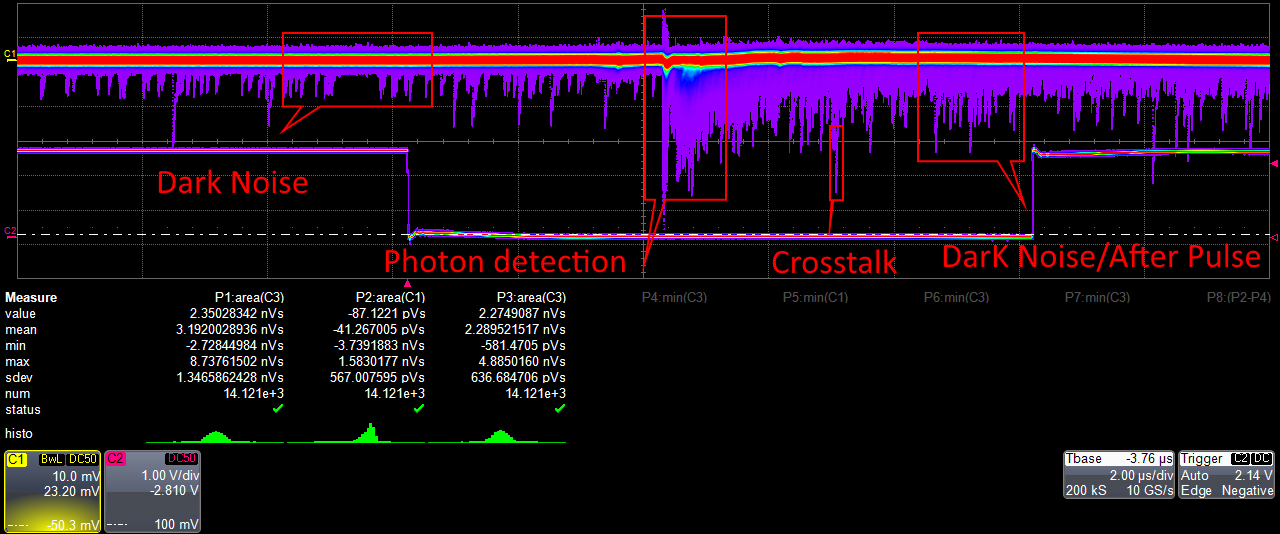
\includegraphics[totalheight=0.2\textwidth,trim=0.3cm 6.6cm 0.1cm 0cm, clip=true]{../Pictures/Pictures_oscilloscope/DN_AP_CT_1.jpg}
    \caption{Les trois probl\`emes principaux. L'axe horizontal est le temps (1$\Pmu$s/div), l'axe vertical est la tension (10mv/div).}
    \label{fig:DN_AP_CT}
  \end{figure}
  
\paragraph{\textit{\underline{Notre exp\'erience}}}
  \leavevmode
  \\
  
  Pour rester proche des conditions exp\'erimentales de nEXO, notre exp\'erience consiste en une boite en aluminium contenant une 
  lampe falsh au X\'enon ainsi qu'un syst\`eme de refroidissement permettant de travailler \`a $-100^\circ$C.\\
  Un filtre plac\'e devant la lampe permet de s\'electionner la longueur d'onde de 175 nm et d'autres filtres identiques att\'enuent la lumi\`ere. 
  Le faisceau se s\'epare ensuite en deux \`a l'aide d'un s\'eparateur de faisceau. L'un des faisceau va irradier la surface d'un premier photo-d\'etecteur 
  (VUV2 SiPM), non refoidi.L'autre fera de m\^eme sur un deuxi\`eme photo-d\'etecteur (VUV3 SiPM) refoidi \`a $-100^\circ$C. 
  Le premier permet de v\'erifier si la quantit\'e de lumi\`ere re\c cue par la second est constante au cours du temps. Il permet aussi de 
  calculer l'efficacit\'e absolue du second. Il s'agira de caract\'eriser ce deuxi\`eme photod\'etecteur. Enfin la boite est remplie 
  d'un gaz -N2- afin de permettre la propagation des photons vers 
  les photo-d\'etecteurs mais aussi d'\'eviter la pr\'esence de gel sur la surface du photod\'etecteur refroidi. 
  \\
  
  Cependant un probl\`eme majeur de bruit \'electronique a retard\'e la prise de donn\'ees. En effet la lampe en fonctionnement \'emet des ondes 
  radio qui sont transmises par toutes surfaces m\'etalliques de la boite. Ainsi les deux signaux re\c cue des diff\'erents photod\'etecteurs 
  s'en trouvent d\'eform\'es \`a tel point qu'il n'est plus possible d'identifier les pr\'ec\'edentes impulsions noy\'ees dans ce bruit d'origine 
  \'electronique. Une des solutions fut d'enrouler les fils transportant les impulsions avec une feuille d'aluminium. De cette 
  mani\`ere les amplificateurs sont reli\'ees \`a la terre via une des pates des photod\'etecteurs.
  
\paragraph{\textit{\underline{L'efficacit\'e quantique}}}
  \leavevmode
  \\
  
  La lampe est allum\'ee sur une p\'eriode de 10$\Pmu$s, avec une fr\'equence de r\'ep\'etition de 100Hz. Pendant cette p\'eriode, elle envoie 
  un flash d'une dur\'ee d'environ 1.4$\Pmu$s apr\`es plus de 4$\Pmu$s de chargement. L'\'ecran de l'oscilloscope, et donc chacun des
  signaux enregistr\'es \footnote{Un signal enregistr\'e correspond \`a une capture d'\'ecran de l'oscilloscope}, est divis\'e en deux zones
  de 3$\Pmu$s chacune.
  La premi\`ere, dite ``zone
  de lumi\`ere'' est situ\'e apr\`es que la lampe a envoyé un flash (\`a partir de 4$\Pmu$s). Dans cette zone les impulsions primaires 
  peuvent \^etre soi d\'eclanch\'ees par des photons soi \`a cause du bruit thermique. La deuxi\`eme, dite ``zone d'ombre'', est situ\'ee avant 
  que la lampe ait envoy\'e un flash (avant 4$\Pmu$s). Dans cette zone les implusions primaires ne peuvent \^etre d\'eclench\'ees que par le bruit 
  thermique avec le m\^eme probabilit\'e que dans la ``zone de lumi\`ere''. 
  \\
  
  L'efficacit\'e quantique se mesure donc de cette mani\`ere:
  
  \begin{equation}
    <PE> =  -ln(\frac{P_{L0}}{P_{D0}}), 
  \end{equation}
 
  o\`u $<PE>$, $P_{L0}$ and $P_{D0}$ sont le nombre moyen de photon-\'electrons, la probabilit\'e de n'observer aucune impulsion dans la ``zone 
  de lumi\`ere`` et celle d'en observer aucune dans la ''zone d'ombre``, respectivement.\\
  Cependant les mesures de l'efficacit\'e effectu\'ees pour un photo-d\'etecteur -VUV3 SiPM- dans les m\^emes conditions exp\'erimentales, donnent 
  des r\'esultats diff\'erents. Si certains parma\`etres \footnote{Position et tension de lampe, quantit\'e de N2, poussi\`ere sur la surface des 
  photod\'etecteurs} ont \'et\'e test\'e, le mauvais alignement du faisceau lumineux avec la surface des photod\'etecteurs semble en \^etre la cause 
  principale. Cet effet s'amplifie au fur et \`a mesure que la structure supportant le s\'eparateur de faisceau se refroidit lorsque le 
  syst\`eme de refroidissement impose une temp\'erature de $-100^\circ$C au photod\'etecteur \`a caract\'eriser.
  
  \begin{figure}[!hbtp]
  \centering
  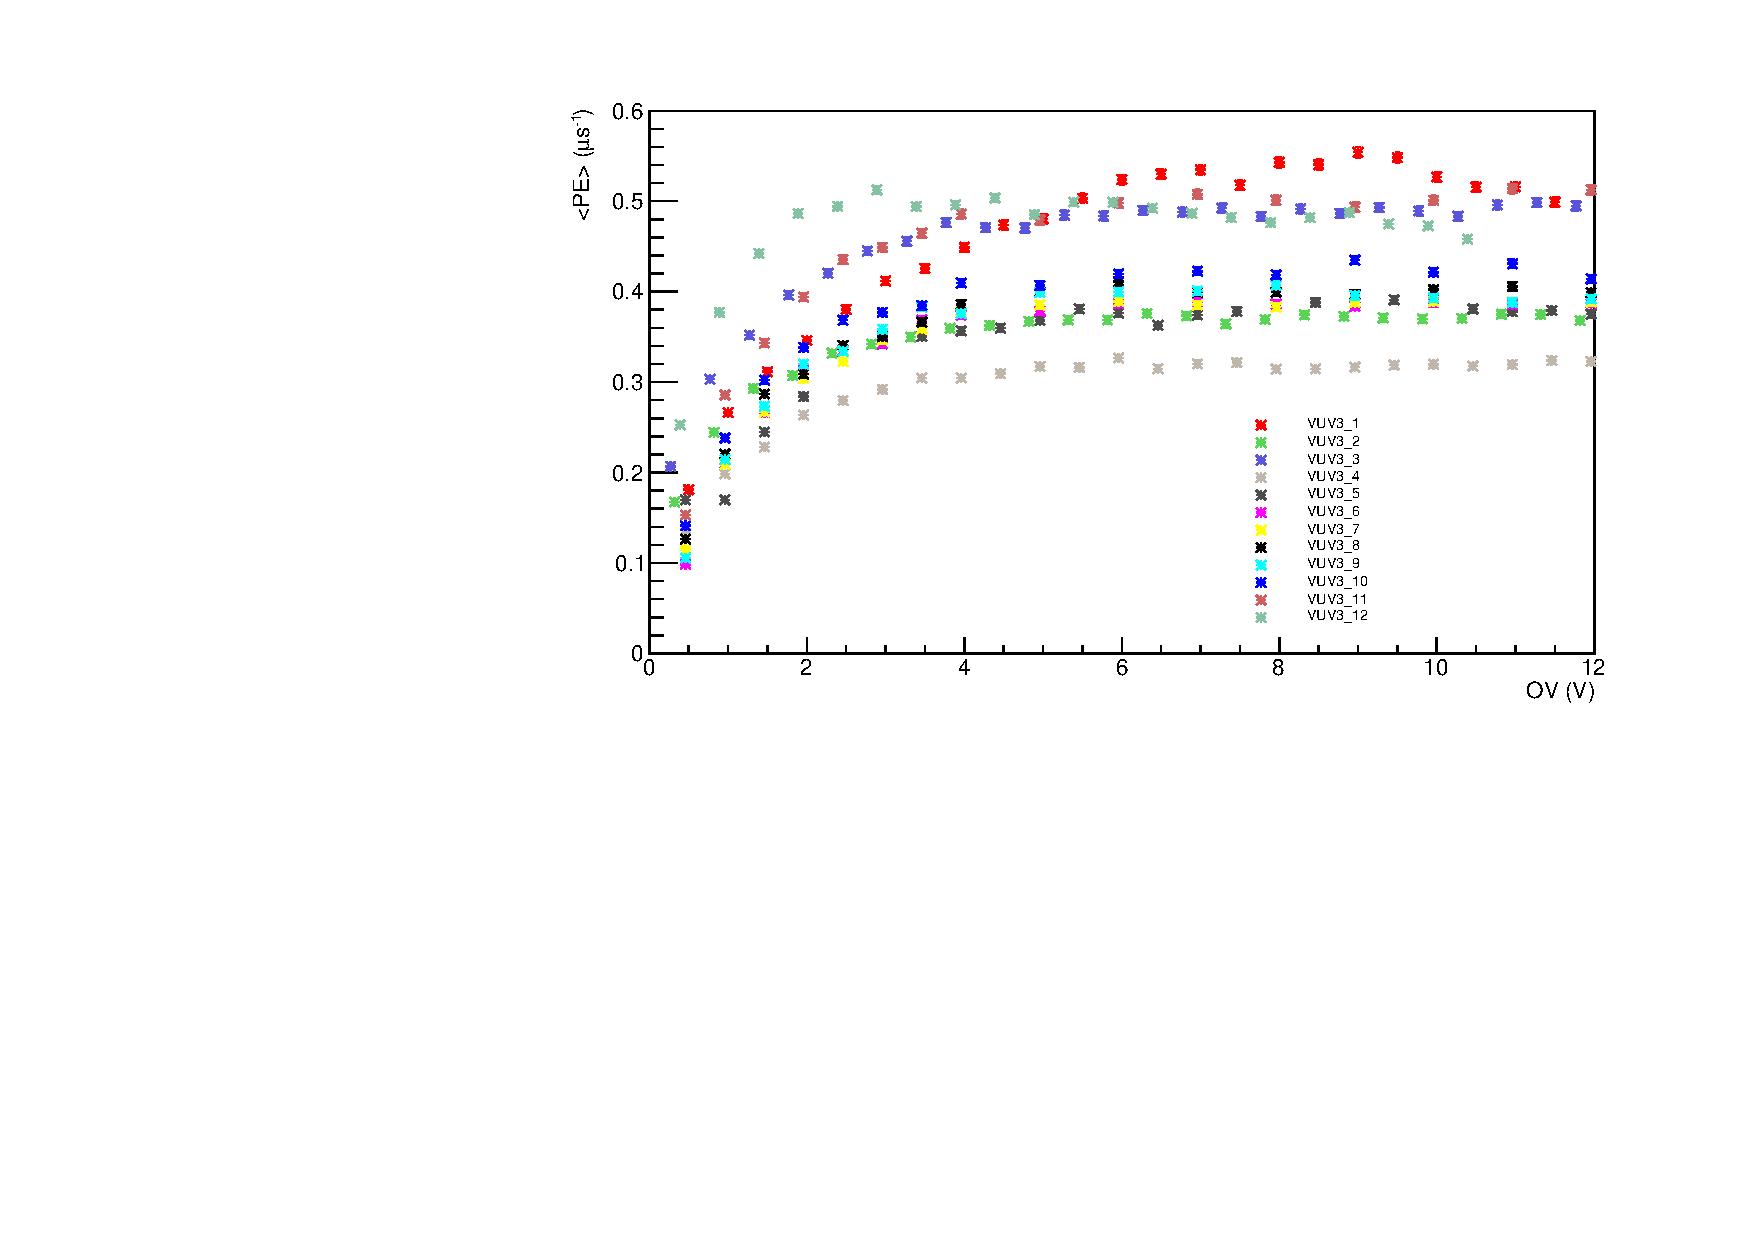
\includegraphics[totalheight=0.35\textwidth,trim=0.5cm 0cm 1.8cm 0.5cm, clip=true]{../Pictures/VUV3_paul.pdf}
  \caption{Les mesures de l'efficacit\'e $<PE>$ ne sont pas reproductibles \`a $-100^\circ$C.}
  \label{fig:issue}
  \end{figure}
  
\paragraph{\textit{\underline{Le bruit thermique}}}
  \leavevmode
  \\
  
  La m\^eme logique des deux zones est utilis\'ee pour calculer le nombre moyen d'implusions d\'eclench\'ees par du bruit thermique. Afin 
  d'augmenter la probabilit\'e d'observer du bruit thermique et d'\'eviter la r\'egion de 1.4$\Pmu$s \footnote{L\`a o\`u les photons de la lampe 
  apparaissent}, les deux zones sont restreintes \`a 1$\Pmu$s chacune et s\'epar\'ees de 4$\Pmu$s.\\
  Le taux de bruit thermique (qui est le bruit thermique par seconde par unit\'e de surface millim\'etrique) $<DN>$ se calcule donc de cette mani\`ere :
  
  \begin{equation}
    <DN> = \ln{\frac{1}{2}\cdot(P_{D0}+P_{L0})}
  \end{equation}
  
  Ce taux en fonction de la temp\'erature \footnote{Du faite que ce bruit soit g\'en\'er\'e thermiquement} ainsi qu' en fonction de 
  l'exc\`es de tension (OV) \footnote{Information extraite de la m\'ethode d' interpolation} sont repr\'esent\'es:  
 
  \begin{figure}[!hbtp]
  \centering
    \begin{subfigure}[Le taux de bruit thermique du d\'etecteur \textcolor{blue}{VUV3 SiPM} et du \textcolor{red}{MEG MPPC}.]{%
      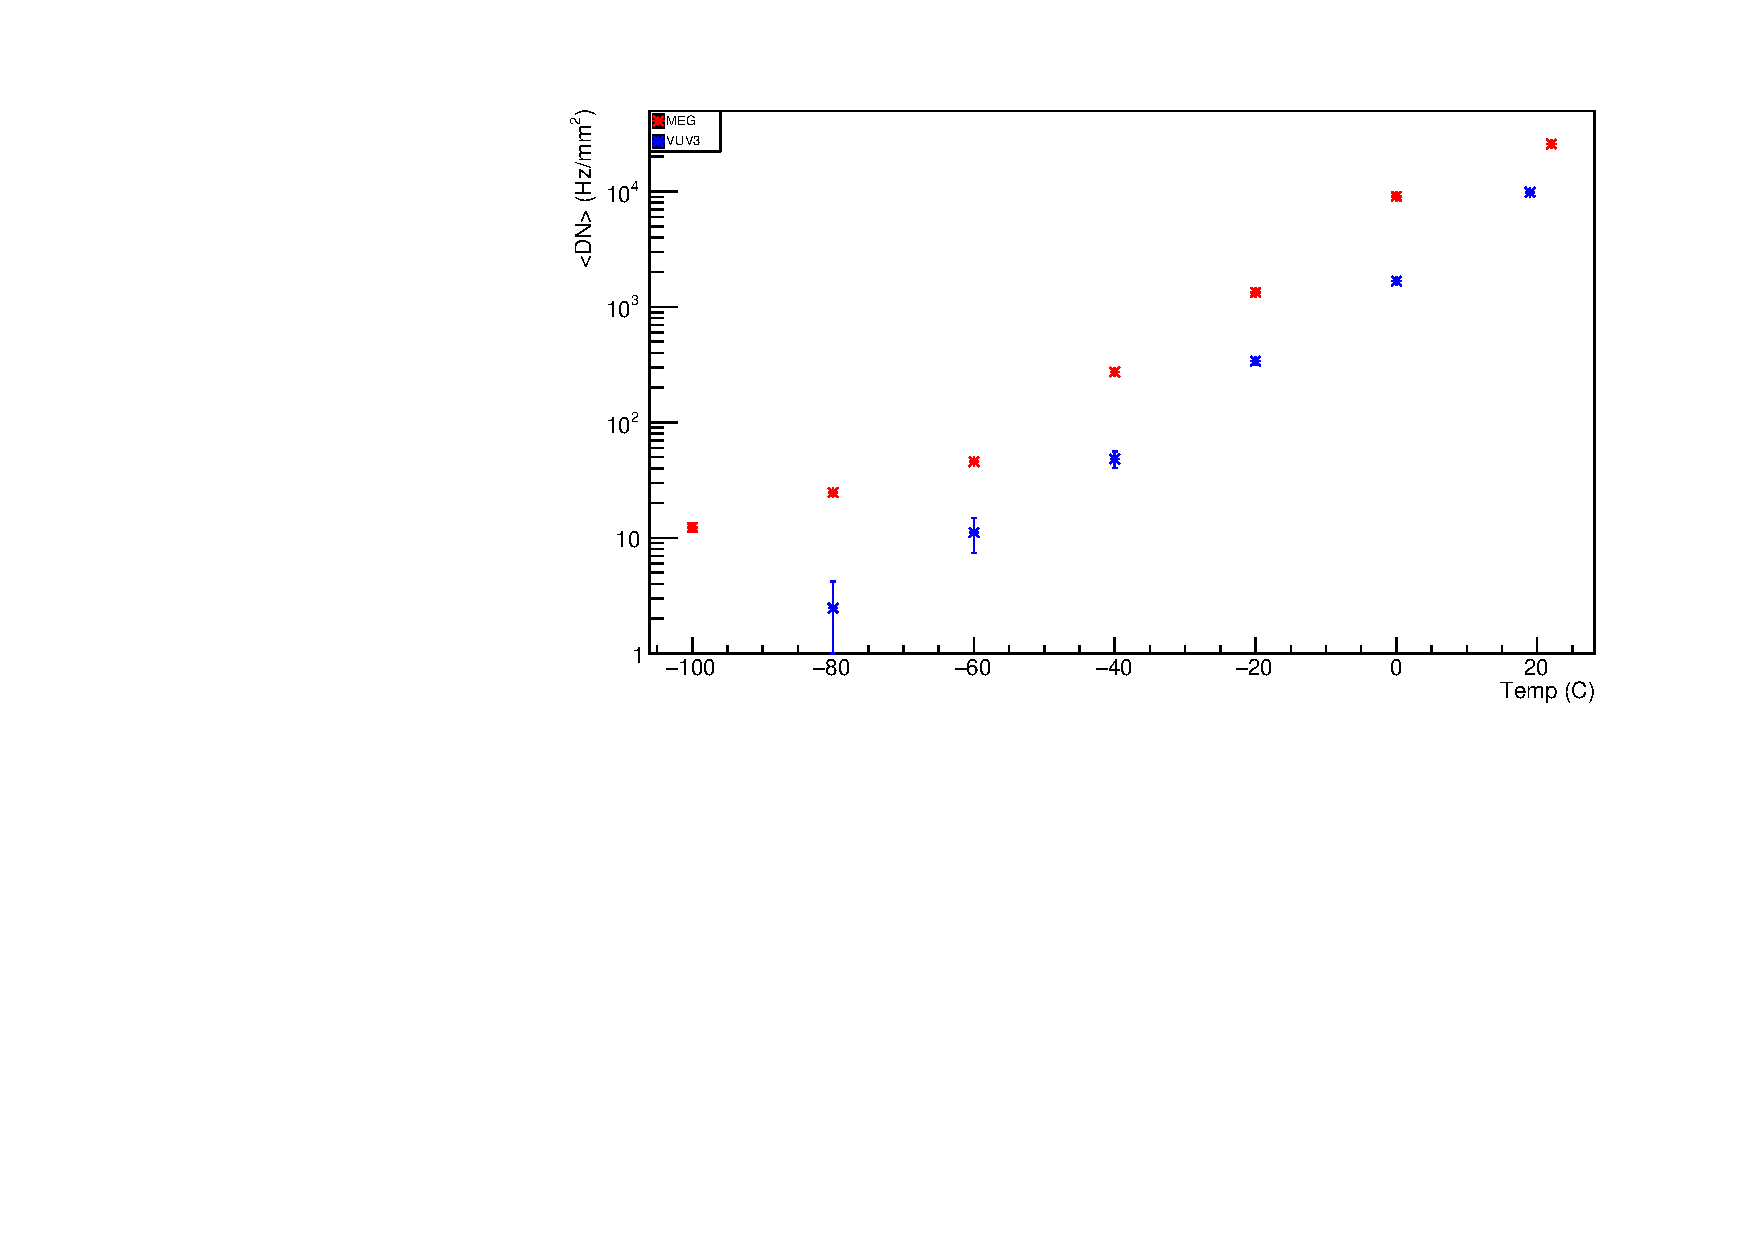
\includegraphics[totalheight=0.3\textwidth,trim=0cm 0cm 1.8cm 0.6cm, clip=true]{../Pictures/DNJuly23.pdf}
      \label{fig:DN_vs_temp}}
    \end{subfigure}
  \quad  
    \begin{subfigure}[Ce m\^eme taux en fonction l'OV pour le VUV3 SiPM \`a $-100^{\circ}$C.]{%
      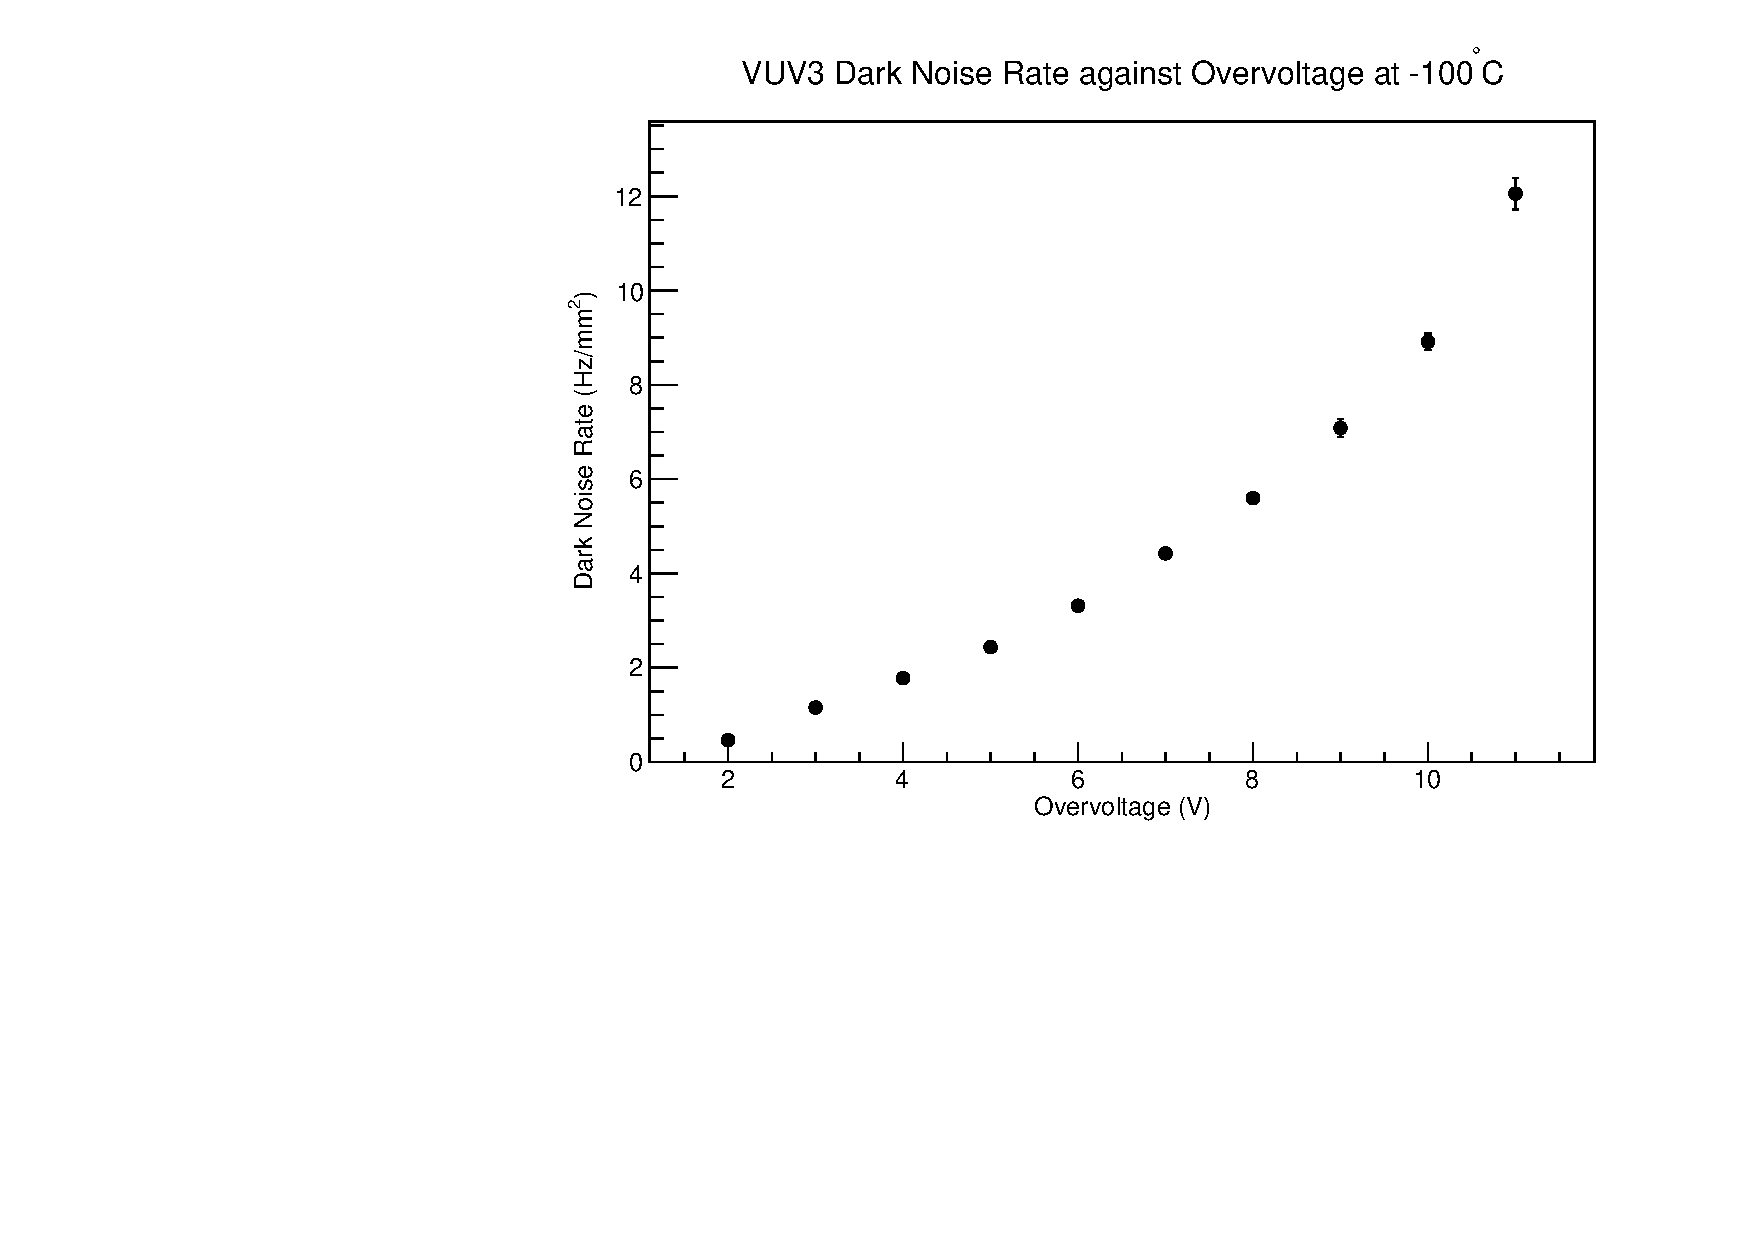
\includegraphics[totalheight=.3\textwidth,trim=.5cm 0cm 1.8cm 1cm, clip=true]{../Pictures/VUV3_DN_vs_OV.pdf}
      \label{fig:DN_vs_OVl}}
    \end{subfigure}
  \caption{Pour le VUV3 SiPM le taux de bruit thermique est inf\'erieur \`a 12Hz/mm\textsuperscript{2}.}
  \label{fig:DN_tem_OV}
  \end{figure}
  
  \newpage
  
\paragraph{\textit{\underline{Les avalanches corr\'el\'ees}}}
  \leavevmode
  \\
  
  Comme le nom l'indique, les avalanches corr\'el\'ees ne peuvent \^etre produites qu'\`a partir d'une impulsion primaire. 
  Pour mesurer le nombre moyen d'impulsions d'interf\'erence $<CT>$, l'id\'ee est de d\'eclencher l'enregistrement du signal provenant d'un 
  photod\'etecteur sur la d\'etection d'une impulsion et non plus sur la d\'etection d'un flash provenant de la lampe. Faisant appara\^itre 
  les impulsions au centre de l'\'ecran, une zone de 200ns est d\'efinie par rapport \`a ce centre.De plus l'amplitude des impulsions 
  d'interf\'erence est le double de celle des impulsions primaires.\\
  Le nombre moyen d'implusions d'interf\'erence se calcule ainsi :
  
  \begin{equation}
    <CT> = -\ln(\frac{N_{1PE}}{N_{>1PE}}),
  \end{equation}
  
  o\`u $N_{1PE}$ et $N_{>1PE}$ sont respectivement le nombre d'impulsions primaires et le nombre total d'impulsions en comptant \`a 
  partir de $N_{1PE}$ (inclu).Comme la probabilit\'e d'observer des impulsions d'int\'eference augmente avec l'exc\`es de tension (OV) 
  appliqu\'ee au photod\'etecteur, il est logique de repr\'esenter $<CT>$ en fonction de OV \ref{fig:CA}.
  
  De plus un algotithme permet de compter le nombre d'implusions \`a partir de la premi\`ere impulsion du premier signal enregistr\'e
  (sur 15000 par exmple). Cette m\'etode de comptage permet donc de tracer la probabilit\'e d'observer une post-impulsion en fonction
  du temps \ref{fig:next_pulse}. Deux formes distinctes s\'epar\'ees \`a 50$\Pmu$s sont assez remarquables. Toutes les  impulsions avant 
  50$\Pmu$s sont consid\'er\'ees comme \'etant des post-impulsions alors que celles apr\`es 
  50$\Pmu$s sont consid\'er\'ees comme \'etant des impulsions primaires g\'en\'er\'ees thermiquement.\\
  Par ailleurs \`a partir de 50$\Pmu$s il est possible d'extraire le nombre moyen de post-impulsions $<AP>$ ainsi que le taux de bruit 
  thermique $<DN>$. C'est la m\'ethode d'interpolation:
  
  \begin{equation} \label{eq:fitting_AP_DN}
    P_{total} = P_{0AP}\cdot <DN>\cdot\mathrm{e}^{-<DN>\cdot t},
  \end{equation}

  o\`u $P_{0AP}$ est la probabilit\'e de pas observer de post-impulsion et $<DN>$ d\'efinie pr\'ec\'edemment.  
  En combinant les r\'esultas de la m\'ethode de comptage et ceux d' interpolation pour les post-impulsions, on obtient \ref{fig:fitting_counting}:  
  
  \begin{figure}[!hbtp]
  \centering
    \begin{subfigure}[La probabilit\'e d'observer une impulsion apr\`es la premi\`ere impulsion primaire du premier signal enregistr\'e.]{%
      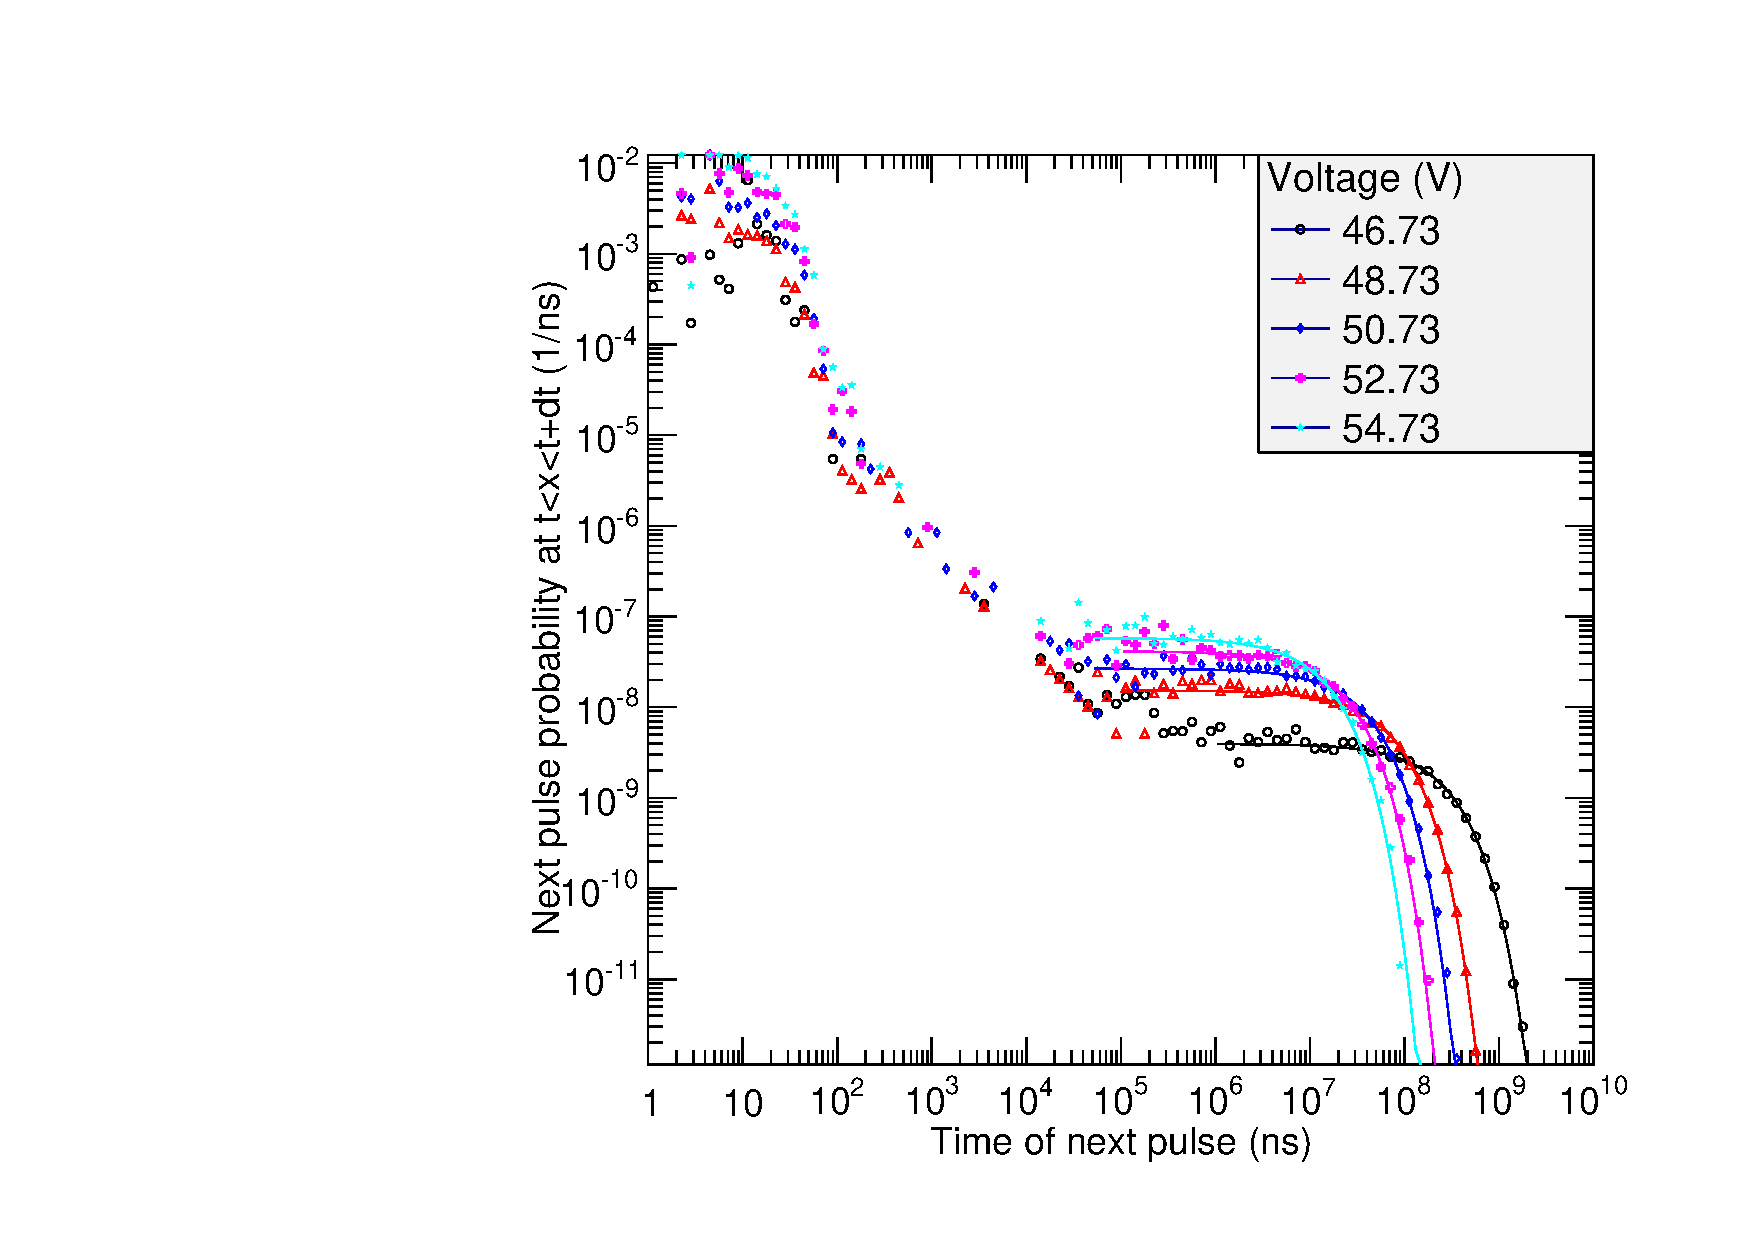
\includegraphics[totalheight=0.35\textwidth,trim=0cm 0cm 1.8cm 0.9cm, clip=true]{../Pictures/deltatime.pdf}
      \label{fig:next_pulse}}
    \end{subfigure}
  \quad  
    \begin{subfigure}[Les deux m\'ethodes donnent les m\^emes r\'esultats pour diff\'erents OV pour le VUV3 SiPM \`a $-100^{\circ}$C.]{%
      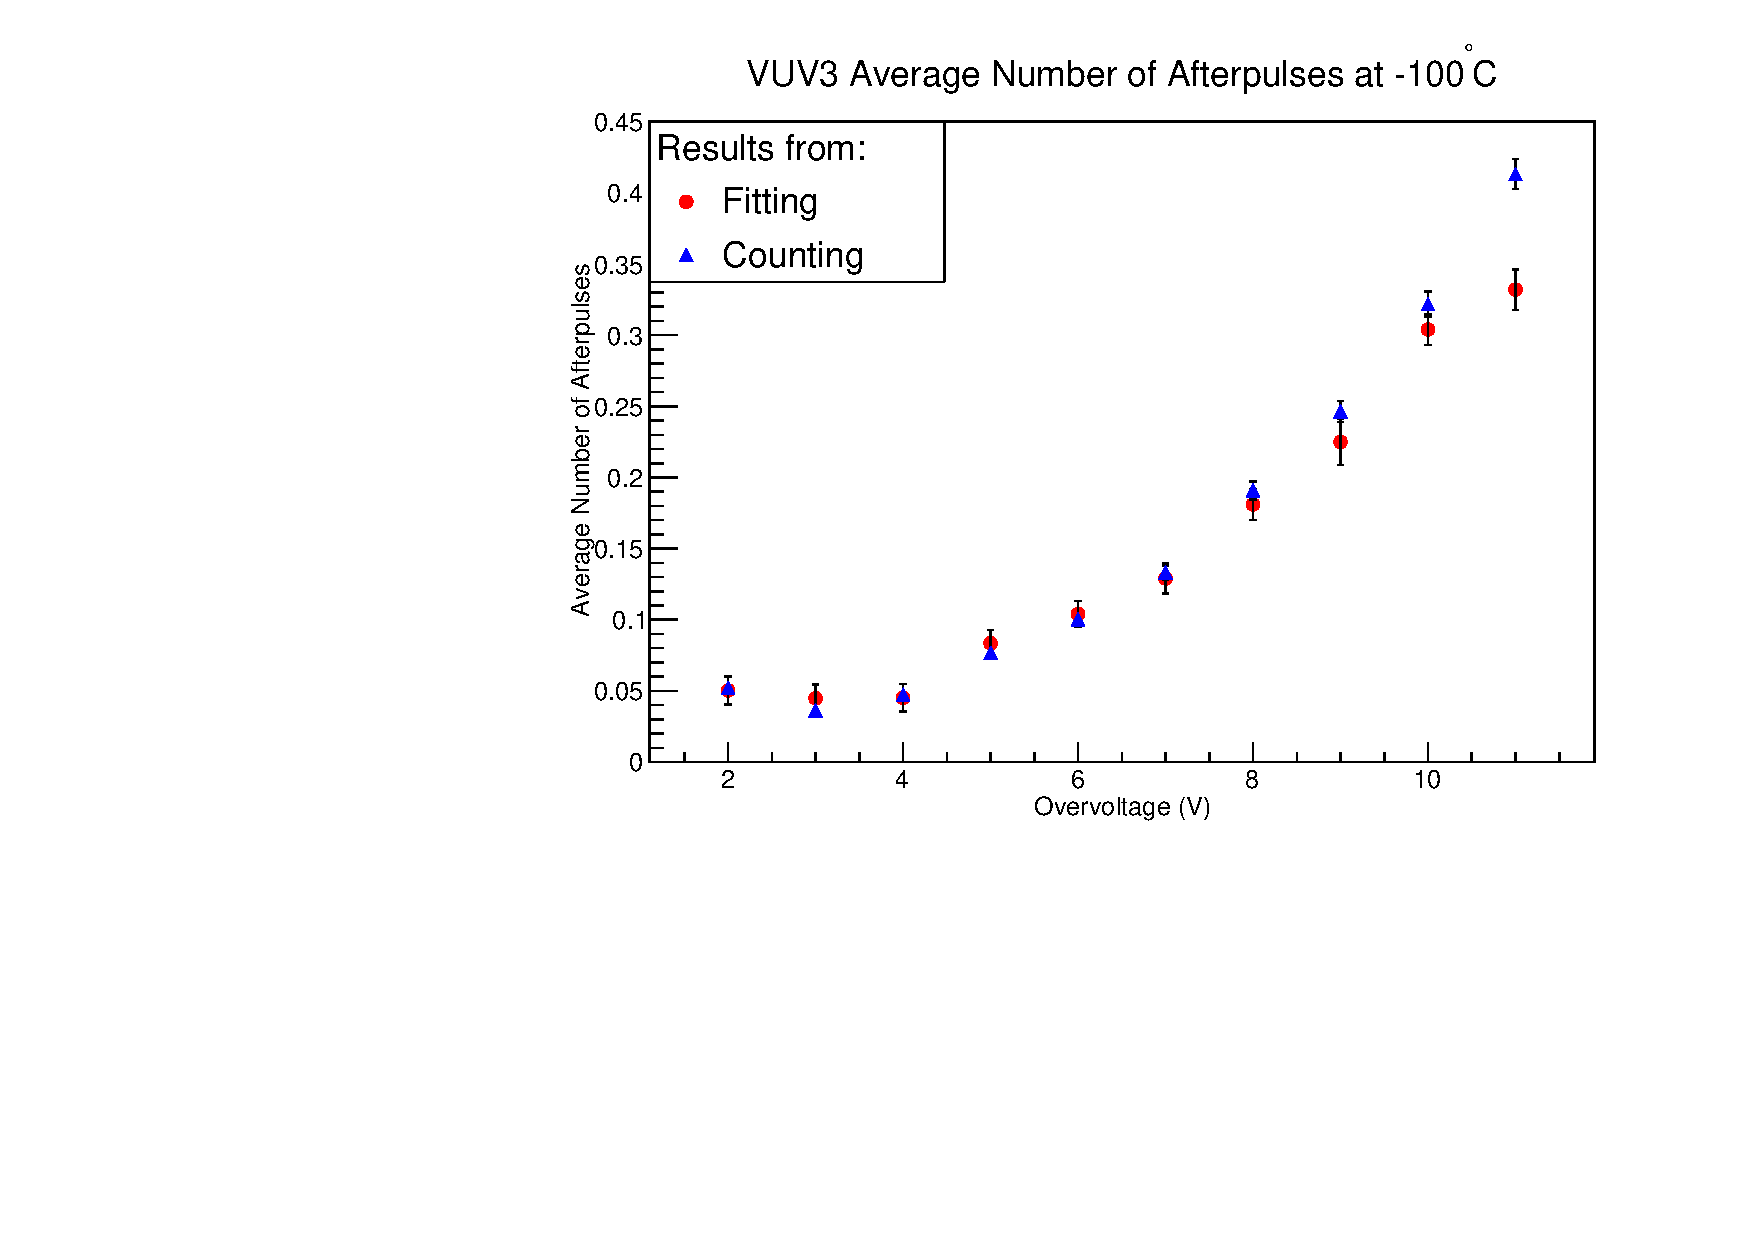
\includegraphics[totalheight=.35\textwidth,trim=.5cm 0cm 1.8cm 0.9cm, clip=true]{../Pictures/VUV3_AP2_vs_OV.pdf}
      \label{fig:fitting_counting}}
    \end{subfigure}
  \caption{Comptage et interpolation donnent le nombre de post-impulsions.}
  \label{fig:next_pulse_pulse_ampl}
  \end{figure}
   
  \newpage
  
  Enfin addionner $<CT>$ et $<AP>$ donne le nombre moyen d'impulsions corr\'el\'ees \`a une impulsion primaire:
  
  \begin{figure}[!hbtp]
    \centering
    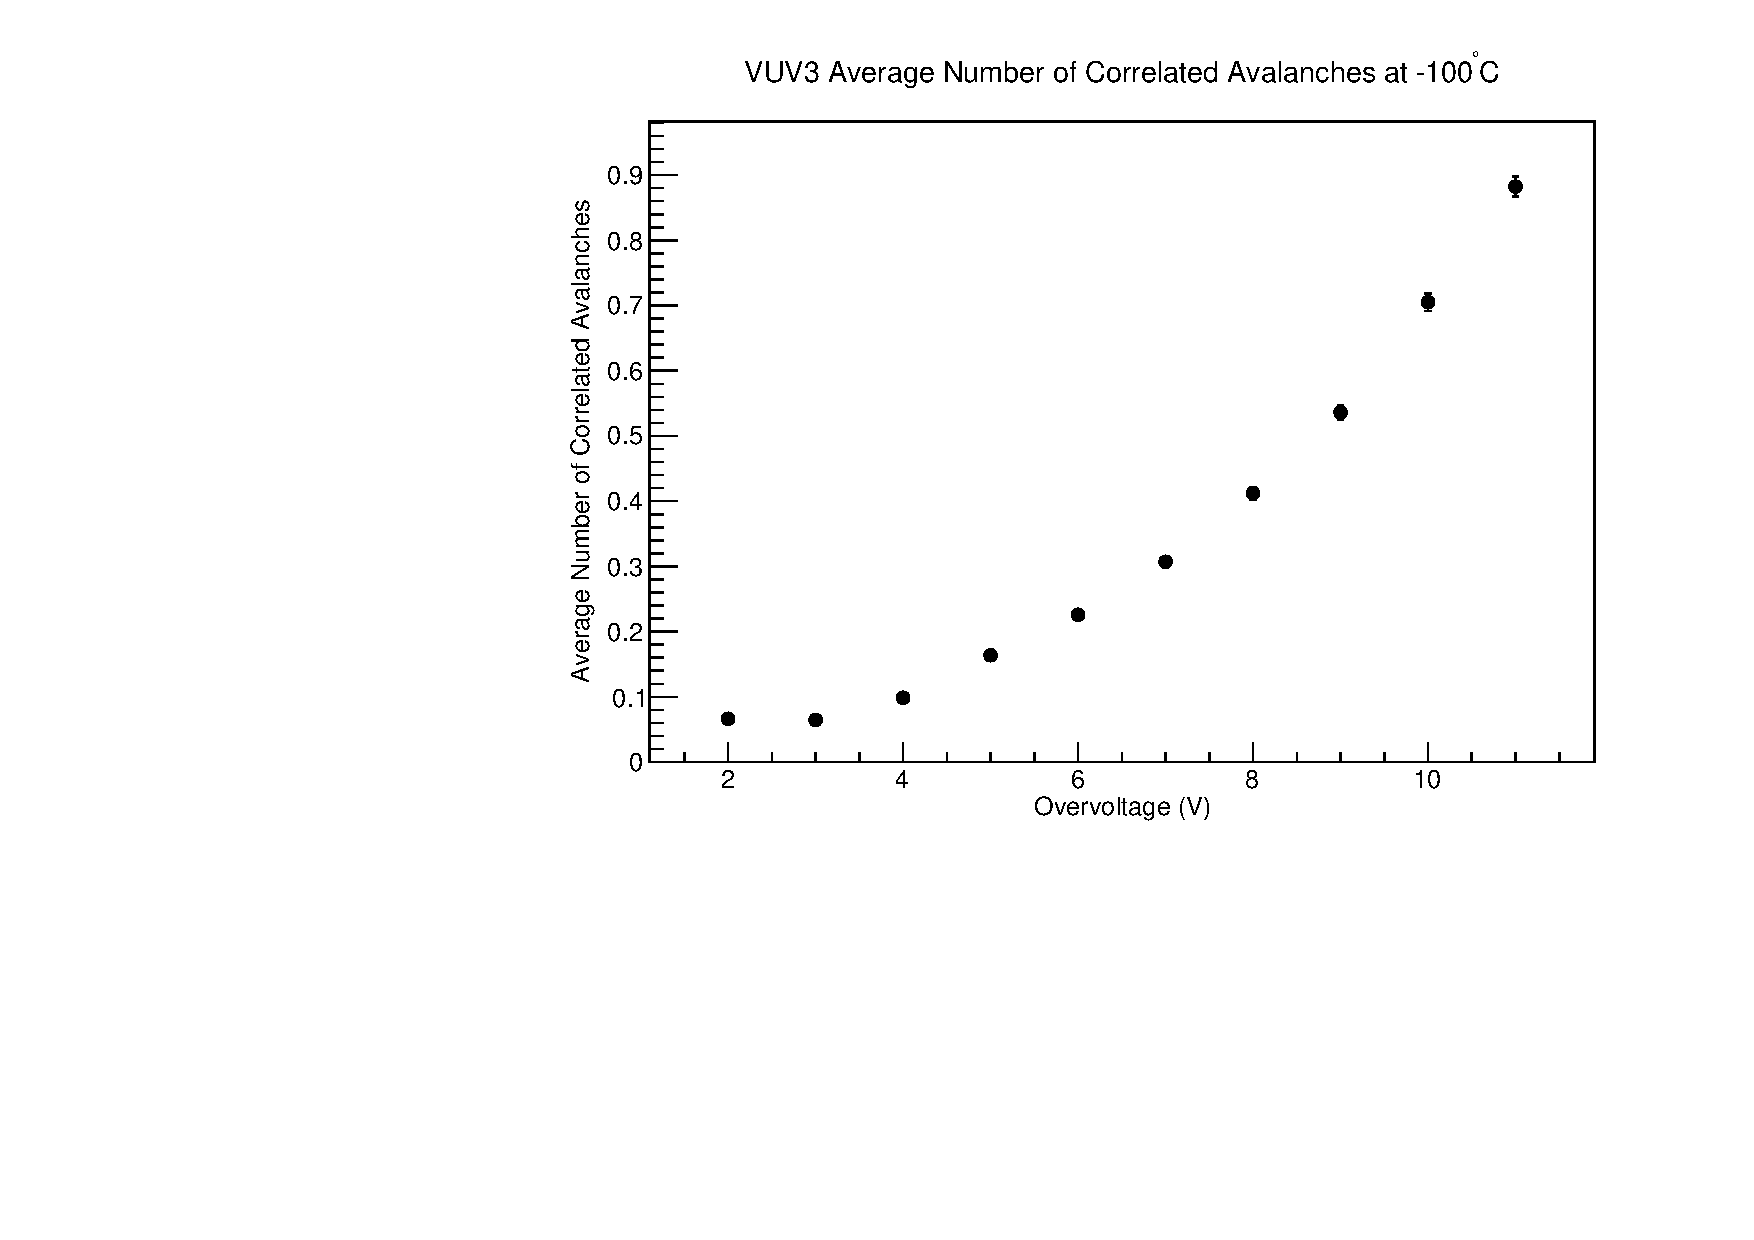
\includegraphics[totalheight=0.35\textwidth,trim=.5cm 0cm 1.8cm 0.9cm, clip=true]{../Pictures/VUV3_CA_vs_OV.pdf}
    \caption{Le nombre moyen d'impulsions corr\'el\'ees pour le VUV3 SiPM \`a $-100^{\circ}$C.}
    \label{fig:CA}
  \end{figure}
  
  
\paragraph{\textit{\underline{Conclusion et recommendations}}}
  \leavevmode
  \\
  
  Bien que la mesure de l'efficacit\'e quantique soit un des buts premiers du stages, le mauvais alignement de la lampe avec les photod\'etecteurs
  ne permet pas de le faire. Nous recommendons d'agrandir le faisceau avec une lentille. 
  \\
  
  Cependant les r\'esultats prometteurs pour le VUV3 SiPM int\'eresseront l'exp\'erience nEXO puisque le taux de bruit thermique par seconde et par 
  unit\'e de 
  surface millim\'etrique est moins de 12Hz/mm\textsuperscript{2} \`a $-100^{\circ}$C et que le nombre moyen d'impulsions 
  corr\'el\'ees est moins de 0.2 per impulsion primaire, et ceci jusqu'\`a une exc\`es de tension de 5V \`a cette temp\'erature. 
  Nous recommendons de confirmer des r\'esultats pour d'autres photo-d\'etecteurs (MEG MPPC, coated SiPM, FBK). 
  
\end{document}

%%%%%%%%%%%%%%%%%%%%%%%%%%%%%%%%%%%%%%%%%%%%%%%%%%%%%%%%%%%%
%%%%%%%%%%%%%%%%%%%%%%%%%%%%%%%%%%%%%%%%%%%%%%%%%%%%%%%%%%%%
%%%%%%%%%%%%%%%%%%%%%%%%%%%%%%%%%%%%%%%%%%%%%%%%%%%%%%%%%%%%
%%%%%%%%%%%%%%%%%%%%%%%%%%%%%%%%%%%%%%%%%%%%%%%%%%%%%%%%%%%%
%%%%%%%%%%%%%%%%%%%%%%%%%%%%%%%%%%%%%%%%%%%%%%%%%%%%%%%%%%%%


remplacer avec Ctrl + R, une fois que le document est fini de r\'edig\'e.
caract\`eres :
'	'
à	\`a
â	\^a
é	\'e
è	\`e
ê	\^e
ù	\`u
ô	\^o
î	\^i
ï	\"i
ç	\c c
œ	\oe{}
²	\texttwosuperior{}
>	\textgreater
"	\og	(ouvrant)
"	\fg{}	(fermant)

